
	\documentclass[oneside]{VUMIFPSkursinis}
\usepackage{algorithmicx}
\usepackage{algorithm}
\usepackage{algpseudocode}
\usepackage{amsfonts}
\usepackage{float}
\usepackage{amsmath}
\usepackage{bm}
\usepackage{caption}
\usepackage{color}
\usepackage{float}
\usepackage{graphicx}
\usepackage{listings}
\usepackage{subfig}
\usepackage{wrapfig}
\usepackage[%  
    colorlinks=true,
    linkcolor=black
]{hyperref}
\university{Vilniaus universitetas}
\faculty{Matematikos ir informatikos fakultetas}
\department{Programų sistemų katedra}
\papertype{Laboratorinis darbas I}
\title{Automatinė ūkio valdymo sistema}
\titleineng{Automatic farm management system}
\status{2 kurso 3 grupės studentai}
\author{Matas Savickis}
\secondauthor{Justas Tvarijonas}  
\thirdauthor{Greta Pyrantaitė}   
\fourthauthor{Rytautas Kvašinskas}
\supervisor{Karolis Petrauskas, Doc., Dr.}
\date{Vilnius – \the\year}

% Nustatymai
%\setmainfont{Palemonas}   % Pakeisti teksto šriftą į Palemonas (turi būti įdiegtas sistemoje)
\bibliography{bibliografija}

\begin{document}
\maketitle

\tableofcontents


\centering	
\sectionnonum{Įvadas}
Automatinė ūkio valdymo sistema (toliau - Auto ūkis) yra programa, leidžianti ūkininkui valdyti jo ūkį skaitmeniniu būdu. Auto ūkis leidžia registruoti gyvūnus ir stebėti kiekvieno jų bioparametrus (kraujo spaudimą, svorį, sveikatą) bei matyti ūkio technikos judėjimą po žemės plotą. Taip pat sistema vartotojui leidžia sekti dirvos parametrus (drėgmę, pH lygį), oro prognozes ir gyvūnų ligų paplitimą aplinkinėse teritorijose. Auto ūkis padeda ir su verslo valdymu: nesunkiai galima samdyti darbuotojus, atlikti buhalterinę apyskaitą, stebėti rinkos kainas ir apskaičiuoti bei numatyti galimą pelną. Iškilus nelaimei per Auto ūkio sistemą galima greitai iškviesti greitąją pagalbą, policiją, gaisrinę ar saugos tarnybą. Orų prognozės yra paimtos iš www.gismeteo.lt. Pagrindinė sistemos inovacija yra tai, kad, kai sistema yra pilnai įdiegta, darbuotojų skaičius, reikalingas palaikyti ūkį, tampa minimalus. Kadangi ūkio technika būtų valdoma automatiškai, vairuotojų ir derliaus nurinkėjų nereiktų. Gyvūnų sekimas yra įgyvendinamas mikro kontrolerio su Arduino pagalba. Šis kontroleris nedidelis ir lengvai pritaikomas visokio pobūdžio darbams. Jį, kartu su WiFi moduliu, sistema naudoja gauti gyvūno lokaciją per Google Maps,- taip pasiklydę ar pavogti gyvūnai būtų greitai surandami ir grąžinami. Žemės laistymas ir tręšimas taip pat būtų automatizuotas: parametrai gaunami per Arduino detektorius, kurie pagal pasikeitusią dirvos kompoziciją nusprendžia, ko trūksta žemei, ir aktyvuoja laistymo ir tręšimo sistemas. Darbuotojų samdymas yra įgyvendintas per darbo biržos puslapį, kur greitai ir nesunkiai galimą įdėti skelbimą arba surasti darbuotoją. Buhalterija yra tvarkoma naudojantis nemokama buhalterijos programa Wave Accounting, kuri yra implementuota į Auto ūkį.  Auto ūkio sistema yra parašyta JAVA kalba - tai leidžia programą paleisti ant bet kurios operacinės sistemos. Ateityje numatoma galimybė programą perkelti į išmaniuosius telefonus. Sistema buvo projektuojama pasitelkiant www.planttext.com ir www.draw.io funkcionalumą.

\section{Sukurtos sistemos aprašymas(v1.0)}

\subsection{Loginis pjūvis}
\subsubsection{Žodynas}
\begin{itemize}
	\item Klasės:
		\begin{itemize}
			\item[*] AutoUkis - pagrindinė (main) programos klasė. Ši klasė piešia grafinę vartotojo sąsają ir laiko savyje kitų klasių objektus, kurių informacija reikalinga piešimui.
			\item[*] Map - teritorijos piešimui skirta klasė.
			\item[*] ZemesTeritorija - apskaičiuoja tam tikros teritorijos plotą.
 			\item[*] Gyvunas - klasė, skirta gyvūno rodmenims ir metodams saugoti.
			\item[*] AriamasLaukas - laiko savyje reikšmes, apibūdinančias unikalų lauką, ir metodus, susijusius su lauko darbu.
			\item[*] Ganykla - laiko parametrus ir metodus darbui su ganyklomis, kurios yra žemės plote.
			\item[*] UkinisPastatas - saugo ūkinę techniką arba gyvūnus.
			\item[*] UkioTechnika - laiko ūkio technikos duomenis ir apskaičiuoja technikos judėjimo greitį.
			\item[*] ZemesParametrai - saugo įvairius žemės parametrus (drėgmė, pH...).
			\item[*] Orai - klasė, skirta gauti vartotojui reikalingas orų prognozes iš www.gismeteo.lt.
			\item[*] ZemesDetektorius - klasė, skirta bendrauti su žemės detektoriumi.


		\end{itemize}
	\item Bendri terminai:
		\begin{itemize}
			\item[*] Žemės plotas - vieta, kurią valdo ir gali stebėti vartotojas(ūkininkas). 
			\item[*] Detektorius - Arduino mikro kontroleris.
			\item[*] Ūkininkas - žmogus, kurio valdomoje teritorijoje įdiegtas Auto ūkis.
			\item[*] Arduino - mikro kontroleris, skirtas ūkio sekimui.
			\item[*] Automatiškai valdoma - valdymui nereikalinga žmogaus pagalba.
			\item[*] Darbuotojas - žmogus, dirbantis ūkininko versle.
			\item[*] Gyvūnas - visi gyvūnai, kurie priklauso ūkininkui, ir yra registruoti Auto ūkis sistemoje.
		\end{itemize}
\end{itemize}

\pagebreak

\subsubsection{Klasių diagrama}
Pagal suprogramuotą šabloninį programos karkasą nubraižėme  \hyperref[fig:uml]{\textit{ UML diagramą(1 pav)}} minėta PlnatText programa.
	\begin{figure}[H]	
	\centering	
		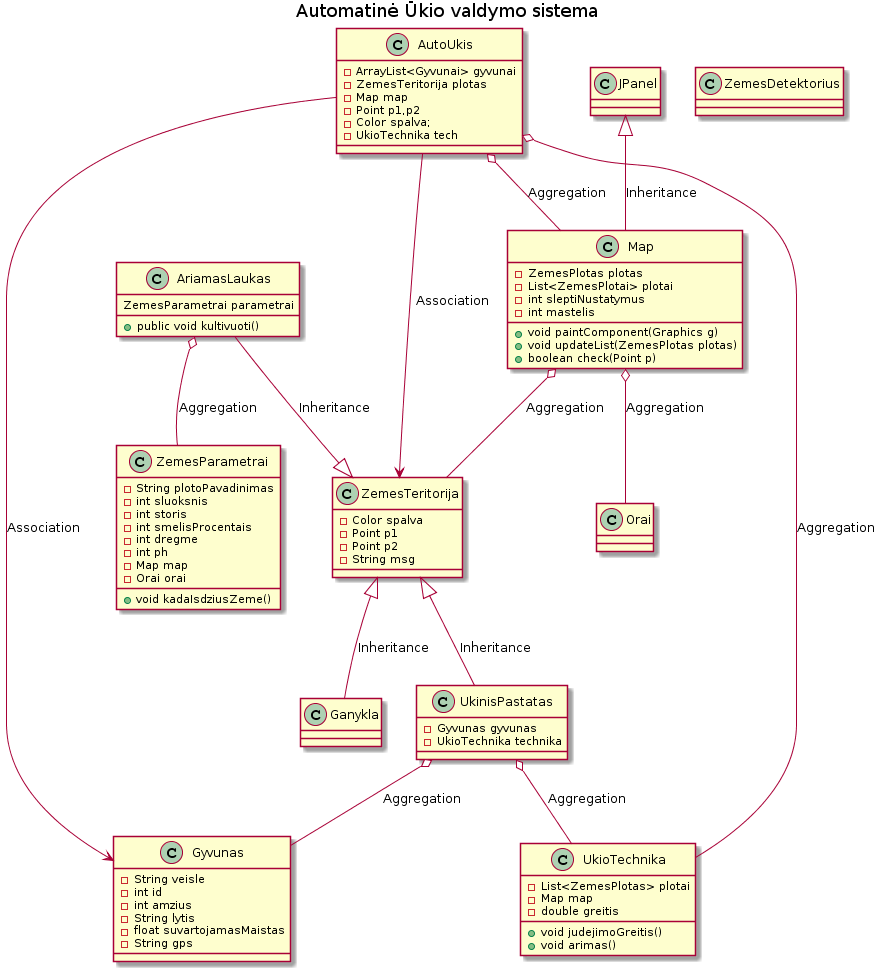
\includegraphics[width=\textwidth,height=\textheight,keepaspectratio]{uml.png}	
		\caption{}
		\label{fig:uml}
	\end{figure}

	
	\pagebreak
	\begin{itemize}
		\item Dizainas: 
		\begin{itemize}
			\item Pagrindinė klasė yra AutoUkis.form. Joje sukurtas ir aprašytas Graphical User Interface (GUI) ir visas vartotojo bendravimas su programa vyksta per ją, nes per ją pasiekiami visi duomenys iš kitų klasių, pavyzdžiui, duomenys, esantys klasėje Gyvūnas, kurioje įrašoma vartotojo įvesta informacija apie gyvūną (veislė, amžius, t.t.). Taip pat AutoUkis klasėje kuriama dauguma objektų ir jie ten laikomi, sudedami į sąrašus. Visos kitos klasės turi savo atskiras paskirtis, tokias kaip žemėlapio braižymas, oro prognozių sekimas ir įvairių parametrų laikymas. Kai kurios klasės (pvz., ZemesDetektorius) buvo sukurtos vėlesniam panaudojimui, bet šiuo metu nėra įgyvendintos.
Dėl to, ką būtų buvę galima daryti kitaip,- GUI perkėlimas į atskirą klasę padarytų programą skaitomesnę ir tvarkingesnę, būtų lengviau rasti atskirą kodą. Dar viena alternatyva būtų įgyvendinti front-end dalį web aplinkoje, bet šiuo metu nematome tam būtinybės.
		\end{itemize}
		\item Funkcionalumas:
		\begin{itemize}
		\item Viso užsibrėžto programos funkcionalumo įgyvendinti nepavyko. Kai kurios klasės buvo sukurtos ateityje planuojamoms funkcijoms, kurios dar nėra implementuotos. Programa kol kas veikia tik ant kompiuterio ir vienintelis jos bendravimas su internetu yra per Orai klasę, kuri skirta vartotojo pasirinkto miesto orų prognozėms gauti iš gismeteo.lt svetainės. Klasėse Gyvunas, Map, ZemesTeritorija ir iš jos išeinančiose klasėse saugomi atitinkami duomenys apie sukurtus objektus bei aprašyti dar neišplėtoti metodai, tokie kaip žemės teritorijos žymėjimas. Planuojama, kad klasė ZemesDetektorius generuos atsitiktinius parametrus, kurie bus perduoti ZemesParametrai klasei.
Nepilnai įgyvendintas finkcionalumas ir neišbaigtos klasės sukelia nepatogumų aprašant programą, nes sunku braižyti diagramas, suvokti aiškius ryšius tarp komponentų ir vykdomų funkcijų.
		\end{itemize}	
	\end{itemize}
	\pagebreak
\subsection{Kūrimo pjūvis}
\begin{itemize}
\item Dizainas: 
		\begin{itemize}
			\item Pradėjus rašyti programą nepagalvojome apie kūrimo pjūvį ir kaip teisingiau būtų galima pradėti viską. Žiūrint dabar, visa programa buvo pradėta kurti pagal Bottom -> Up principą. Iš pradžių apsirašėme daugybę mažų klasių ir paskui jas bandėme apjungti į didesnę sistemą. Išskyrėme tokius komponentus kaip ūkininkas, programa, orų tarnyba, žemės detektorius ir administratorius. Kiekvienas komponentas turi skirtingas prieigas prie informacijos ir skirtingas funkcijas, reikalingas ūkio visapusiškam funkcionavimui. Kai kurios klasės liko nepanaudotos, nes šiuo metu jos neatrodo pakankamai svarbios pradiniam projekto variantui. Ūkiniko, Admin ir darbuotojo panelės įtrauktos į dokumentaciją norint pavaizduoti skirtingas prieigas prie sistemos.
		\end{itemize}
		\end{itemize}
\begin{figure}[H]
\centering	
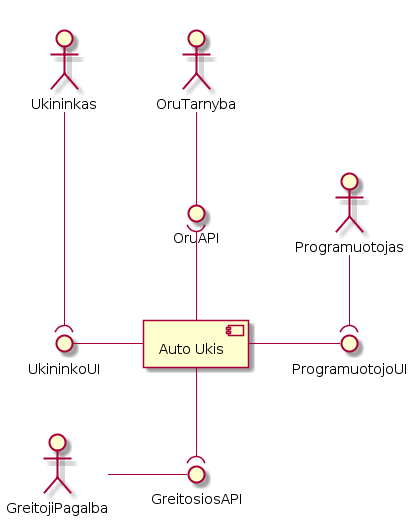
\includegraphics[width=10cm,height=15cm,keepaspectratio]{l0.png}	
\caption{}
\label{fig:l0}
\end{figure}
	\begin{itemize}
		
		\item \hyperref[fig:l0]{\textit{L0}}:
		\begin{itemize}
			\item  \hyperref[fig:l0]{\textit{Šioje diagramoje (2 pav)}} pavaizdavome sistemos bendravimą su išoriniais agentais, tokiais kaip Greitoji pagalba, Ūkininkas ir t.t. . Ši diagrama aiškiai ir paprastai parodo kuriamus ir įgyvendinamus interfeisus. Galbūt būtų galima Greitosios Pagalbos interfeisą išskaidyti į kelis detalesnius interfeisus, bet apskritai didelių problemų nepastebime.

		\end{itemize}

	\end{itemize}
\begin{figure}[H]	
\centering	
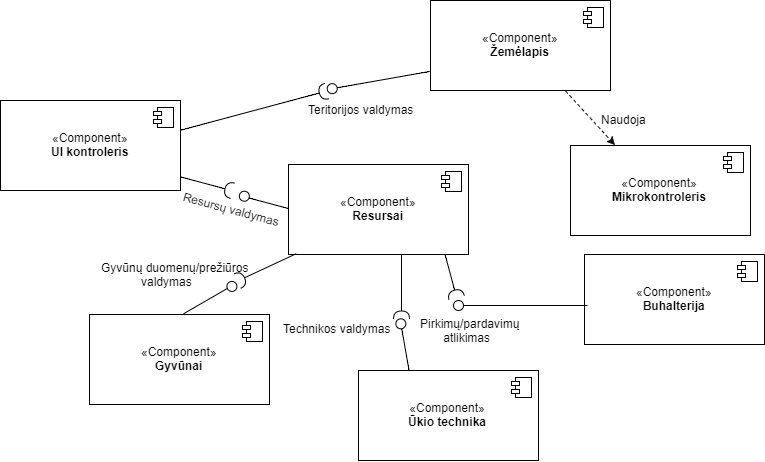
\includegraphics[width=14cm,height=14cm,keepaspectratio]{l1.png}	
\caption{}
\label{fig:l1}
\end{figure}

\begin{itemize}
	\item L1: Sudėjus komandos idėjas apie tai, kaip turėtų atrodyti \hyperref[fig:l1]{\textit{ L1 diagrama(3 pav)}}, supratome, kad mūsų sistema neturi normalios struktūros ir gerai nebuvome pagalvoję kaip visi komponentai siesis vieni su kitais, todėl ir diagrama atrodo chaotiška. Trūksta konkretumo, kaip Admin turi sietis su kitas komponentais. Programa atsiranda kaip komponentas, o tai greičiausiai yra nekorektiška.

\end{itemize}
\begin{figure}[H]
\centering	
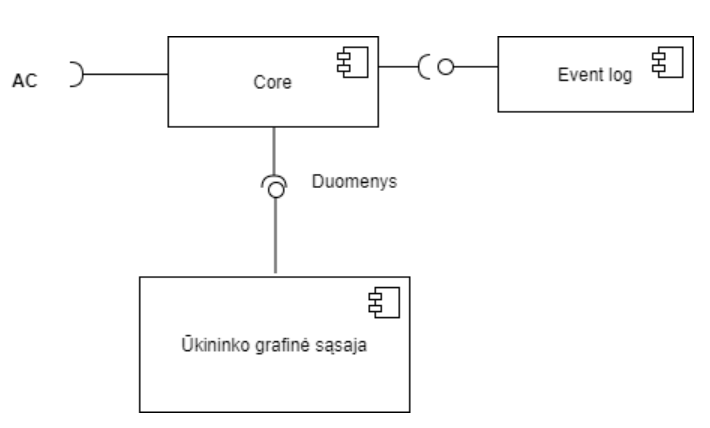
\includegraphics[width=10cm,height=10cm,keepaspectratio]{l2uki.png}
\caption{}
\label{fig:l2uki}
\end{figure}
	

	\begin{itemize}
		\item L2(Ūkininkas):\hyperref[fig:l2uki]{\textit{  Šioje diagramoje (4 pav)}} parodyta, kad programos pagrindas (Core) kuria interfeisą, kuriuo perduoda duomenis grafinei vartotojo sąsajai. Duomenys yra perduodami Event Log komponentui. 

	\end{itemize}
	\begin{figure}[H]
	\centering	
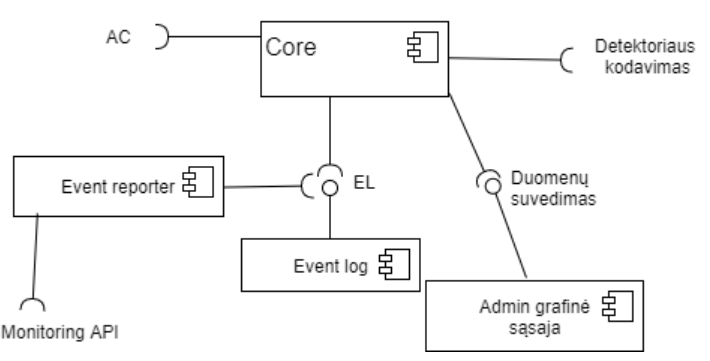
\includegraphics[width=10cm,height=10cm,keepaspectratio]{l2admin.png}
\caption{}
\label{fig:l2admin}
\end{figure}
	
	
	\begin{itemize}
		\item L2(Admin)\hyperref[fig:l2admin]{\textit{  Šioje diagramoje (pav 5)}}  parodyta, kad programos pagrindas naudoja duomenų suvedimo interfeisą, kurį suteikia Admin grafinė sąsaja, bei naudoja Detektoriaus kodavimo interfeisą. Visus įvykius įrašo į Event Log.

	\end{itemize}
	\begin{figure}[H]
	\centering	
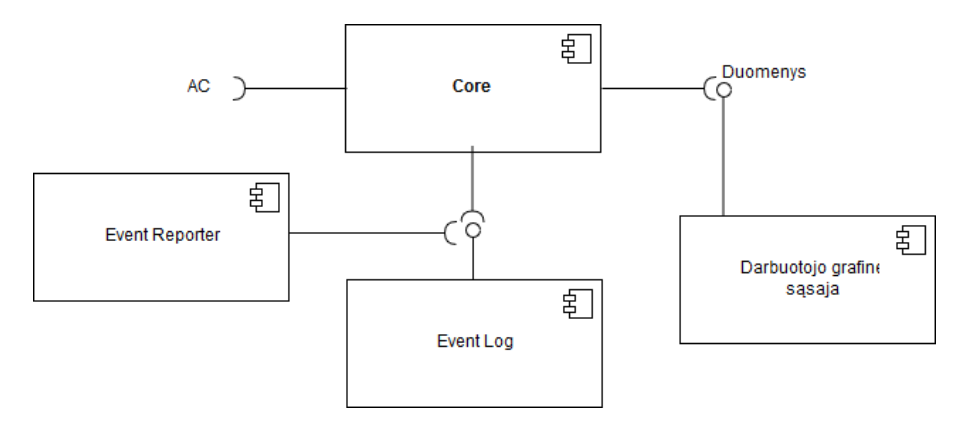
\includegraphics[width=10cm,height=10cm,keepaspectratio]{l2darb.png}
\caption{}
\label{fig:l2darb}
\end{figure}
		

\begin{itemize}
		\item L2(Darbuotojas):\hyperref[fig:l2darb]{\textit{  Šioje diagramoje (pav 6)}}  parodyta, kad programos pagrindas naudoja grafinę sąsają ir perduoda duomenis į Event Log’ą. 
\end{itemize}
\begin{figure}[H]
\centering	
	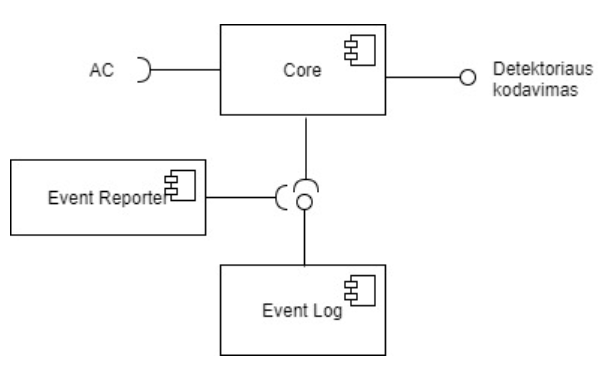
\includegraphics[width=10cm,height=10cm,keepaspectratio]{l2det.png}
	\caption{}
	\label{fig:l2det}
\end{figure}
		
\begin{itemize}
		\item L2(Detektorius):\hyperref[fig:l2det]{\textit{ Ši diagrama (pav 7)}} vaizduoja detektoriaus išvedamus duomenis. Įvykiai įrašomi Event Log’e.
\end{itemize}

	\begin{figure}[H]
	\centering	
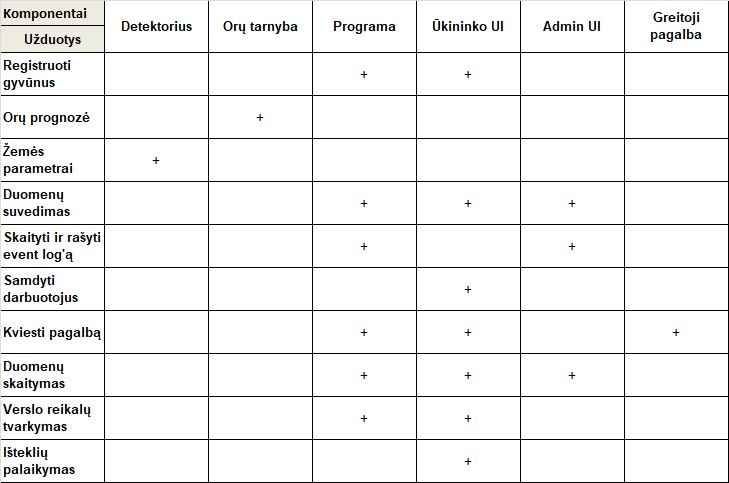
\includegraphics[width=15cm,height=15cm,keepaspectratio]{elementu_ir_uzd_matrica.png}
\caption{}
\label{fig:elementu_ir_uzd_matrica}
\end{figure}
\begin{itemize}
		\item Elementų ir užduočių ryšių matrica(8 pav).
\end{itemize}

\pagebreak
		


\subsection{Use cases}
\begin{itemize}
\item Prisijungimo ir registracijos Use Case(9 pav):
\begin {figure}[H]
	\centering
		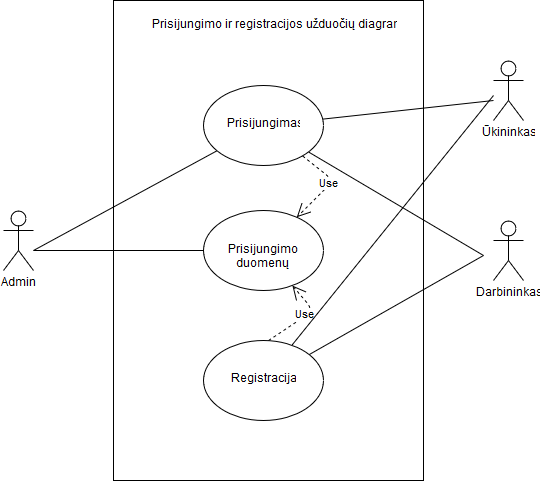
\includegraphics[width=10cm,height=11cm,keepaspectratio]{Use_case_prisijungimas_registracija.png}
	\caption{}
	\label{fig:Use_case_prisijungimas_registracija}
\end{figure}
\item Žemėlapio žymėjimo ir peržiūros Use Case(10 pav):
\begin {figure}[H]
	\centering
		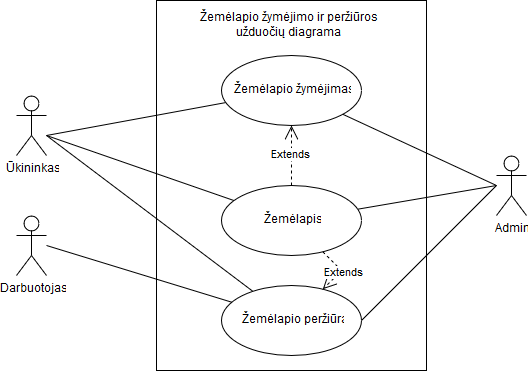
\includegraphics[width=10cm,height=11cm,keepaspectratio]{Use_case_zemelapio_zymejimas.png}
	\caption{}
	\label{fig:Use_case_zemelapio_zymejimas}
\end{figure}

\pagebreak

\item Gyvūnų suvedimo ir peržiūros Use Case(11 pav):
\begin {figure}[H]
	\centering
		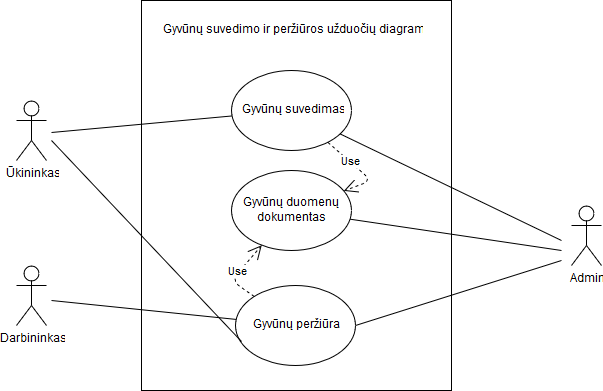
\includegraphics[width=10cm,height=11cm,keepaspectratio]{Use_case_gyvunu_suvedimas.png}
	\caption{}
	\label{fig:Use_case_gyvunu_suvedimas}
\end{figure}
\end{itemize}

\subsection{Proceso pjūvis}
	Šiame skyriuje parodoma programos elgsena jos vykdymo metu.
\subsubsection{Veiklos diagramos}

	Vaizduojama\hyperref[fig:ActivityMapŽimėjimas]{\textit{ Žemėlapio žymėjimo veiklos diagrama (pav 12)}}. Nurodomi pagrindiniai žingsniai braižant žemėlapį.
	\vskip 0.5cm
	\begin{figure}[H]
	\centering	
	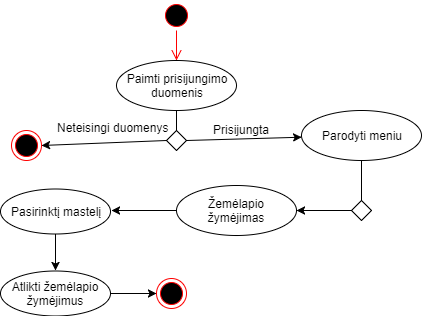
\includegraphics[width=10cm,height=10cm,keepaspectratio]{ActivityMapŽimėjimas.png}
	\caption{}
	\label{fig:ActivityMapŽimėjimas}
\end{figure}

\pagebreak	

\subsubsection{Būsėnų diagrama}
 \hyperref[fig:Busenu]{\textit{Šioje diagramoje (pav 13)}} parodomos galimos vartotojo būsenos ir keliai jom pasiekti. Šiuo metu programoje tėra dvi būsenos, taigi diagrama yra labai paprasta.
	\begin{figure}[H]
	\centering	
	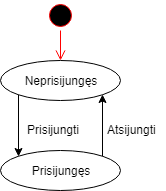
\includegraphics[width=5cm,height=6cm,keepaspectratio]{Busenu.png}
	\caption{}
	\label{fig:Busenu}
\end{figure}
\pagebreak
\subsection{Fizinis pjūvis}
	Šiame skyriuje parodoma (14 pav.) šios sistemos techninė įranga, komunikacija, tačiau, kadangi šioje šabloninėje versijoje nenaudojame kitų techninių resursų be kompiuterio, fizinis pjūvis parodo tik nedidelį kiekį informacijos.
	\newline
	\vskip 0.5cm
	\begin{figure}[H]
	\centering	
	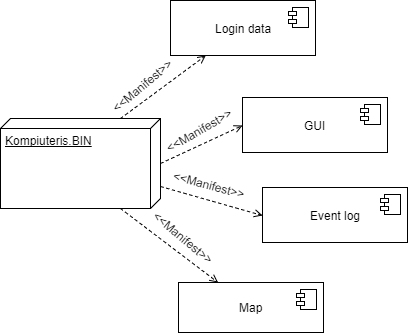
\includegraphics[width=10cm,height=10cm,keepaspectratio]{Deployment.png}
	\caption{}
	\label{fig:Deployment}
\end{figure}
	\begin{itemize}
		\item D0: \hyperref[fig:Deployment]{\textit{Šioje diagramoje(15 pav)}} parodyta, kas saugoma kompiuteryje. 
		Iš diagramos matome, kad šiame įrenginyje saugomi prisijungimo duomenys, vartotojų grafinės sąsajos, teritorijos žemėlapis bei programoje atliktų veiksmų išrašas. Alternatyva buvo saugoti šiuos duomenis išnuomuotame web service, tačiau daug negalvoję nusprendėme duomenis saugoti kompiuteryje.
	\end{itemize}

\pagebreak		

\begin{figure}[H]
		\centering	
	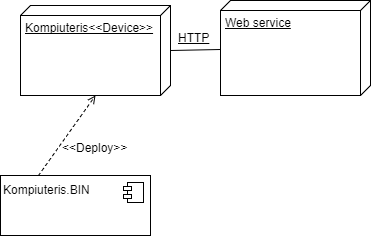
\includegraphics[width=10cm,height=10cm,keepaspectratio]{Deployment0.png}
	\caption{                                                            }
	\label{fig:Deployment0}
\end{figure}
	\begin{itemize}
		\item D1: Tai \hyperref[fig:Deployment0]{\textit{bendresnė D0 diagrama}}, joje matome, kad kompiuteris, norėdamas gauti pranešimus apie orus,  bendrauja su web HTTP ryšiu.
	\end{itemize}

\subsection{Pirmos dalies išvada}
Pirmoji programos versija buvo suprogramuota ir suprojektuota perdaug negalvojant apie sistemos plėtimą ateityje. Nors klasėse ir išlaikėme enkapsuliavimo principą, bendras objektinio programavimo principas nebuvo išlaikytas, klasės yra per daug viena nuo kitos priklausomos. Rimtesniai sistemai kurti reiktų naudotis Top to Bottom principu lengvesniam naujų funkcionalumų pridėjimui. Stipri ir paprasta sistemos dalis pasimato kūrimo pjūvyje, kuriame yra aiškūs ryšiai tarp kuriamų ir įgyvendinamų interfeisų. Aprašinėdami L1 ir L2 supratome, kad nepagalvojome apie tai, kaip sistemos vartotojai bendrauja su sistema. Šią dalį reiks pergalvoti antroje programos versijoje, kad viskas taptų aiškiau ir paprasčiau, reikia labiau pasidomėti, kaip tokios sistemos veikia realiame pasaulyje. Proceso pjūvį pavyko aprašyti pakankamai paprastai ir aiškiai, tačiau jam dar trūksta detalumo ir kitų scenarijų numatymo, pavyzdžiui, kaip prisijungti prie sistemos. Fiziniame pjūvyje aprašyta techninė sistema yra ganėtinai paprasta ir primityvi. Pagrindinis trūkumas - nepagalvota, kas nutiktų kompiuterio išsijungimo atveju, ar kas nutiktų atsiradus poreikiui plėsti sistemą. Žiūrint bendrais idėjos bruožais, brangiausia sistemos dalis yra automatinės mašinos, kurios dar yra sąlyginai nauja technologija, ir mikro kontroleriai kiekvienam gyvūnui. Jeigu ferma turi jų daug, visas instaliavimas kainuotų gana brangiai ir turbūt neatneštų didelės naudos. Tai labiau inovacija dėl inovacijos, ne dėl funkcionalumo. Tačiau kitos dalys visai sėkmingai pritaikomos. Tokią sistemą, kokią padarėme dabar, įgyvendinti būtų įmanoma, tačiau praplėsti ir palaikyti ją būtų nepatogu, ir sistema turbūt nedirbtų taip greitai, kaip norėtųsi. Trūksta funkcionalumo su išmaniuoju telefonu, darbo birža, rinkos tendencijomis ir kita. 

\pagebreak

\section{Perprojektuotos sistemos aprašymas(To-Be, v2.0)}

\subsection{Loginis pjūvis}
\subsubsection{Žodynas}
\begin{itemize}
	\item Klasės:
		\begin{itemize}
			\item[*] AutoUkis - pagrindinė (main) programos klasė. Ši klasė piešia grafinę vartotojo sąsają ir laiko savyje kitų klasių objektus, kurių informacija reikalinga piešimui.
			\item[*] Zemelapis - teritorijos piešimui skirta klasė.
			\item[*] ZemesTeritorija - apskaičiuoja tam tikros teritorijos plotą.
 			\item[*] Gyvunas - klasė, skirta gyvūno rodmenims ir metodams saugoti.
			\item[*] AriamasLaukas - laiko savyje reikšmes, apibūdinančias unikalų lauką, ir metodus, susijusius su lauko darbu.
			\item[*] Ganykla - laiko parametrus ir metodus darbui su ganyklomis, kurios yra žemės plote.
			\item[*] UkinisPastatas - saugo ūkinę techniką arba gyvūnus.
			\item[*] UkioTechnika - laiko ūkio technikos duomenis ir apskaičiuoja technikos judėjimo greitį.
			\item[*] ZemesParametrai - saugo įvairius žemės parametrus (drėgmė, pH...).
			\item[*] Orai - klasė, skirta gauti vartotojui reikalingas orų prognozes iš www.gismeteo.lt.
			\item[*] Detektorius - klasė, skirta bendrauti su žemės detektoriumi.
			\item[*] VartotojoSasaja - programos grafinė vartotojo sąsaja.
			\item[*] Tvartas - pastatas, kuriame laikomi ūkio gyvūnai.
			\item[*] Garazas - pastatas, kuriame laikoma ūkio technika.
			\item[*] Sandelis - sandėlyje laikomi ūkio ištekliai.
			\item[*] Naudotojas - žmogus, kuris naudojasi programa.
			\item[*] SOSPagalba - šioje klasėje iškviečiama pagalba pavojaus atveju.
			\item[*] Ukininkas - žmogus, kurio valdomoje teritorijoje įdiegtas Auto ūkis.
			\item[*] Darbuotojas - žmogus, dirbantis ūkininko versle.
			\item[*] Traktorius - atlieka žemės padargų traukimo funkciją.
			\item[*] Kombainas - nuima grūdų derlių.
			\item[*] Adminas - administratorius, atsakingas už tvarkingą programos veiklą.
			\item[*] SQLUzklausa - uzklausa gauti duomenims iš duombazės.
			\item[*] IsoriniaiServisai - kitos paslaugos (pvz., darbo birža).
			\item[*] RinkosAnalizatorius -  renka duomenis apie rinkos naujienas, aktualias naudotojui.
			\item[*] Saskaita - laikomi sąskaitos duomenys ir funkcijos veiksmam su ja atlinkti.
			\item[*] Finansai - laikoma informacija apie ūkio finansus ir aprašytos funkcijos veiksmam su jais.
			\item[*] Skaiciavimas - atlieka kompleksinius skaičiavimus.
			\item[*] EventReporter - klasė, kuri rašo įvykius į Event Log.
			\item[*] EventLog - įvykių programoje įrašai.

		\end{itemize}
	\item Bendri terminai:
		\begin{itemize}
			\item[*] Žemės plotas - vieta, kurią valdo ir gali stebėti vartotojas (ūkininkas). 
			\item[*] Detektorius - Arduino mikro kontroleris.
			\item[*] Arduino - mikro kontroleris, skirtas ūkio sekimui.
			\item[*] Automatiškai valdoma - valdymui nereikalinga žmogaus pagalba.
			\item[*] Gyvūnas - visi gyvūnai, kurie priklauso ūkininkui, ir yra registruoti Auto ūkis sistemoje.
		\end{itemize}
\end{itemize}

\pagebreak

\subsubsection{Klasių diagrama}
			\begin{figure}[H]
		\centering	
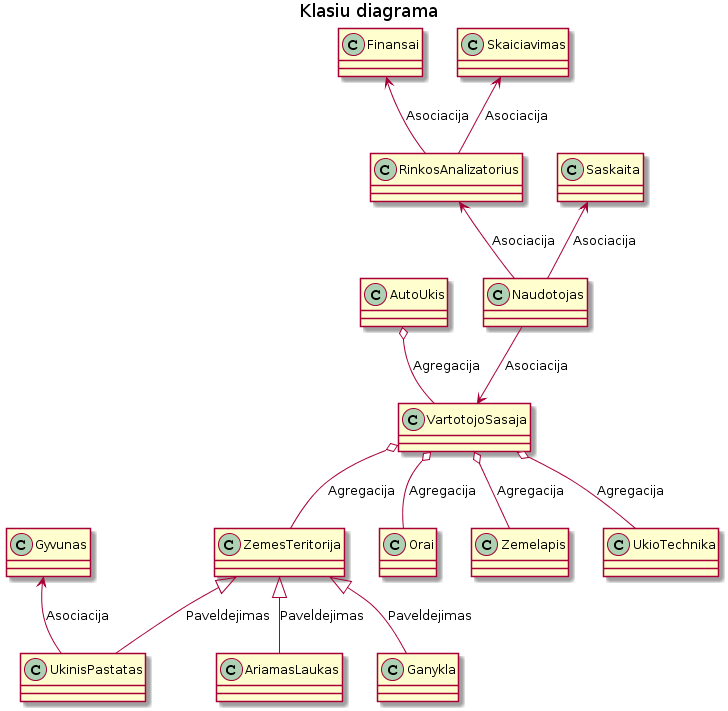
\includegraphics[width=18cm,height=17cm,keepaspectratio]{Klasesv2.png}
	\caption{}
	\label{fig:Klasesv2}
\end{figure}
	
	\begin{itemize}
		\item Dizainas:
			\begin{itemize}
				\item Visas programos dizainas(16 pav) paremtas Top to Bottom principu. Pradėjome galvoti dideliais objektais ir juos išskirstėm į mažesnius. Pagrindinė klasė yra AutoUkis, kuris iškviečia VartotojoSasaja klasę, kuri ir piešia visą prieinamumą vartotojams. Galima nesunkiai pridėti kitokią vartotojo sąsają ar bet kokią kitą UI piešimo galimybę, kaip, pavyzdžiui, piešti UI išmaniajame telefone. Programos modalumas leidžia nesunkiai pridėti funkionalumo, nes programos dalys yra atskiros viena nuo kitos. Pavyzdžiui, ištrynus klasę ŪkinisPastatas visos programos veikimas nesutriktų. 
			\end{itemize}
		\item Funkionalumas: 
			\begin{itemize}
				\item Programos funkcionalumas susideda iš trijų pagrindinių dalių, vartotojų prieiga prie sistemos, finansų bei išteklių (žmogiškųjų ir natūraliųjų) valdymas, išteklių sekimas. Prieigos dalyje funkcionalumas pasižymi prieigos išskaidymu - skirtingi sistemos vartotojai gauna skirtingą prieigą ir galimybes naudotis sistema. Pavyzdžiui, darbuotojas negali tvarkyti įmonės finansų, tačiau visi sistemos vartotojai gali kviesti greitąją pagalbą. Nesunku implementuoti naują vartotojų klasę (pvz. Svečias). Finansų bei išteklių dalyje ūkininkas gali tvarkyti savo išteklius, pavyzdžiui, samdyti arba atleisiti darbuotojus, stebėti rinkos kainą ir nuspręsti, kada jam palankiausia parduoti, sudarinėti sąskaitas ir tvarkyti kitą buhalteriją. Trečiojoje sistemos dalyje yra įgyvendinamas išteklių sekimas. Vartotojai, turintys prieigą gali stebėti žemės parametrus, ūkio technikos sąrašą, ūkinių pastatų sąrašą bei gyvūnų, priklausančių sistemai, sąrašą.
			\end{itemize}

	\end{itemize}

\begin{itemize}
		\item Elementų ir užduočių ryšių matrica:
\end{itemize}
	\begin{figure}[H]
	\centering	
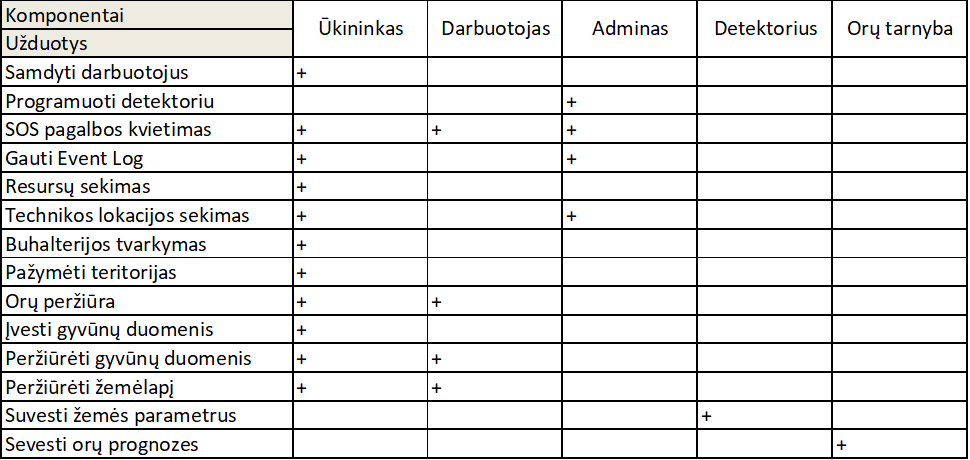
\includegraphics[width=15cm,height=15cm,keepaspectratio]{KomUzd2.png}
\caption{}
\label{fig:elementu_ir_uzd_matrica}
\end{figure}

\pagebreak

\subsection{Kūrimo pjūvis}
	\begin{itemize}
		\item Dizainas:
		\begin{itemize}
			\item Programos dizainas stipriai paremtas Top to bottom projektavimo principu ir objektinio programavimo enkapsuliacijos paradigma. Sistema(18 pav) sukuria ir įgyvendina kitų sistemų intefeisus. Pagrindiniai keturi interfeisai, sukuriami programos, yra UkininkasUI, DarbuotojasUI ir AdminasUI, SOSPagalbaUI. Šie interfeisai suteikia prieigą prie sistemos skirtingas privilegijas turintiems vartojams. Sistema įgyvendina OruAPI kuriam interfeisą.

		\end{itemize}
	\end{itemize}

\begin{figure}[H]
		\centering	
	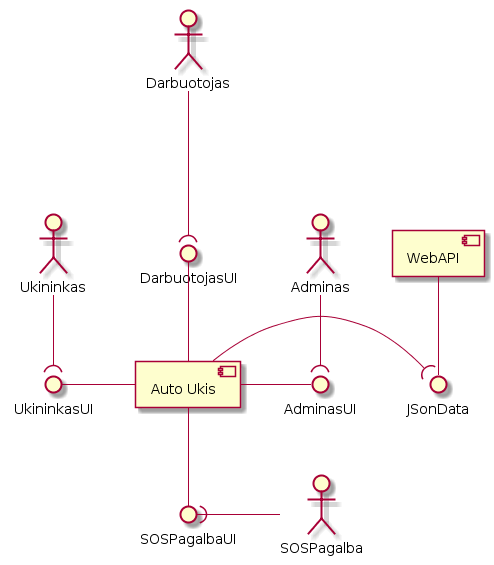
\includegraphics[width=17cm,height=20cm,keepaspectratio]{L0V2.png}
	\caption{}
	\label{fig:L0V2}
\end{figure}
	\begin{itemize}
	\item L0:
	\begin{itemize}
	\item Šioje diagramoje(18 pav) pavaizdavome sistemos bendradarbiavimą su išoriniais agentais, tokiais kaip MikroKontroleris, Ukininkas ir t.t. . Ši diagrama parodo sistemos įgyvendinamus ir kuriamus interfeisus. Iš diagramos matome, kad programos pagrindas kuria interfeisą ne tik vartotojams, bet ir tokiems išoriniams agentams, kaip SOS pagalba ir orų tarnyba.
\end{itemize}
	\begin{figure}[H]
		\centering	
	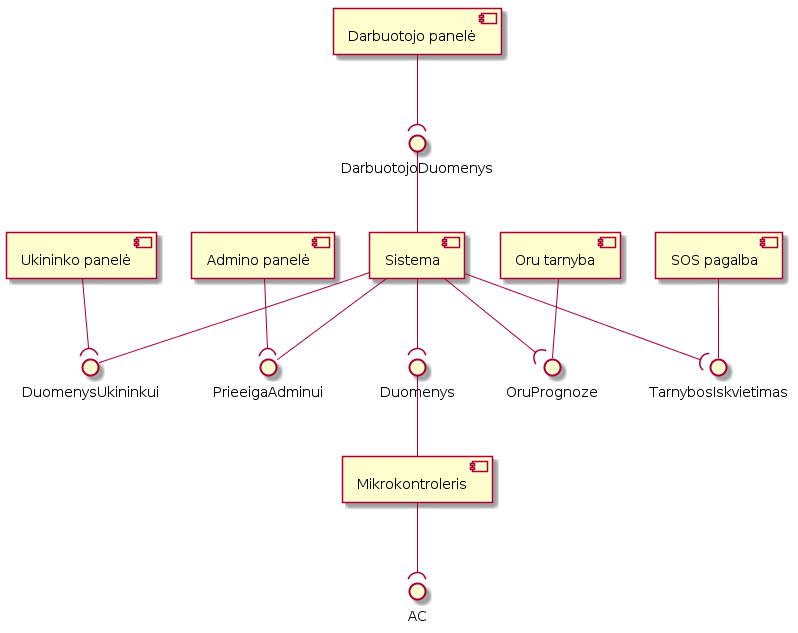
\includegraphics[width=17cm,height=20cm,keepaspectratio]{L1V2.png}
	\caption{}
	\label{fig:L1V2}
\end{figure}
\item L1: Sistemos(19 pav) struktūra ganėtinai aiški. Yra trys panelės, kurios pasiima sisteminius duomenis, ir trys panelės, kurios suteikia duomenis sistemai. Kadangi struktūra paprasta, nesunku prie jos pridėti ar gauti duomenis iš naujų komponentų.
\pagebreak

	\begin{figure}[H]
	\centering	
	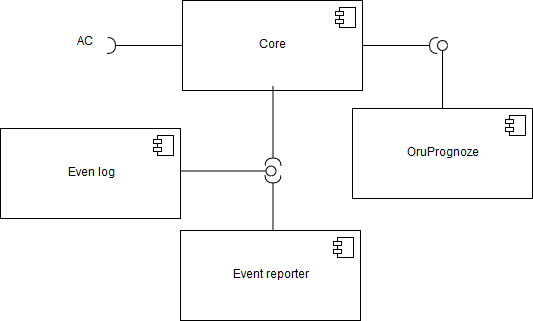
\includegraphics[width=10cm,height=10cm,keepaspectratio]{L2(oruprognoze).png}
	\caption{}
	\label{}
	\end{figure}
	\item L2(Oru prognozė): Šioje diagramoje(20 pav) pavaizduotas Orų prognozės komponento veikimas. Sistema įgyvendina Orų prognozės interfeisą ir perduoda informaciją Event Log'ui. Jame laikoma informacija apie orus, iš kurio reikiamą info gali pasiimti Event reporteris įgyvendindamas Event Log interfeisą.
\begin{figure}[H]
		\centering	
	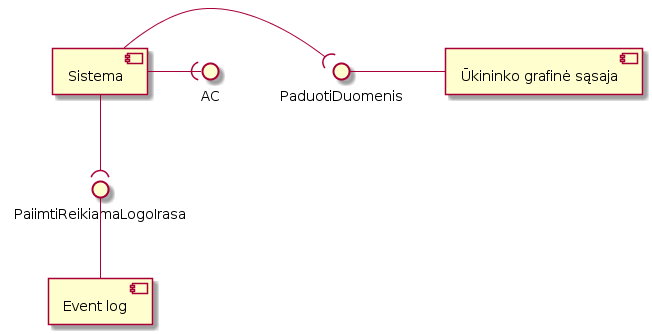
\includegraphics[width=15cm,height=15cm,keepaspectratio]{l2v2uki.png}
	\caption{}
	\label{fig:}
\end{figure}
\item L2(Ūkininkas): Ūkininko panelė(21 pav) gauna informaciją įgyvendindama Sistemos suskurtą interfeisą. Sistema tuo tarpu įgyvendina Event Log kuriamą interfeisą ir paduoda reikiamus duomenis ūkininko UI.
\begin{figure}[H]
		\centering	
	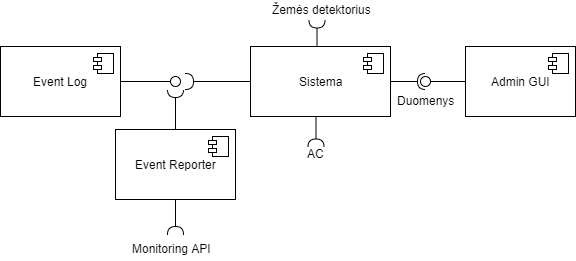
\includegraphics[width=15cm,height=15cm,keepaspectratio]{2L2Admin.png}
	\caption{}
	\label{fig:}
\end{figure}
\item L2(Admin): Diagramoje(22 pav) pavaizduotas Admin panelės bendravimas su sistema. Norėdamas gauti prieigą prie duomenų jis įgyvendina tik vieną Sistemos kuriamą interfeisą. Pati sistema visus duomenis gauna įgyvendindama kitų komponentų kuriamus interfeisus. Sistema įgyvendina Žemės detektoriaus ir Event Log interfeisus, per kuriuos sistema gauna ir vėliau perduoda duomenis Admin GUI.
\begin{figure}[H]
		\centering	
	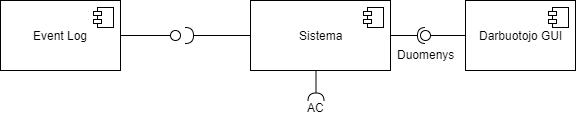
\includegraphics[width=15cm,height=15cm,keepaspectratio]{2L2Darb.png}
	\caption{}
	\label{fig:}
\end{figure}
\item L2(Darbuotojas): Šioje diagramoje(23 pav) pademonstruojamas Darbuotojo GUI bendravimas su sistema. Sistema sukuria interfeisą, kurį įgyvendina Darbuotojas GUI. Jeigu darbuotojui reikia kažkokių duomenų iš Event log ar bendrai iš sistemos, Sistema įgyvendina Event Log interfeisą ir taip paduoda duomenis Darbuotojo GUI. 

	\begin{figure}[H]
		\centering	
	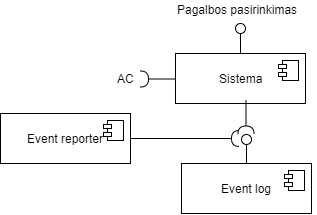
\includegraphics[width=10cm,height=10cm,keepaspectratio]{L2SOS.png}
	\caption{}
	\label{fig:L2SOS}
\end{figure}
\item L2(SOS pagalba):
Šioje diagramoje(24 pav matome, kad Core kuria interfeisą reikiamos pagalbos pasirinkimui, kurį įgyvendins vartotojas iškvietęs SOS pagalbą. Pagalba turi galimybę gauti kažkokius įrašus iš Event Log, susijusius tu kritine situacija. Perdavimas vyksta per Sistema.

	\begin{figure}[H]
	\centering	
	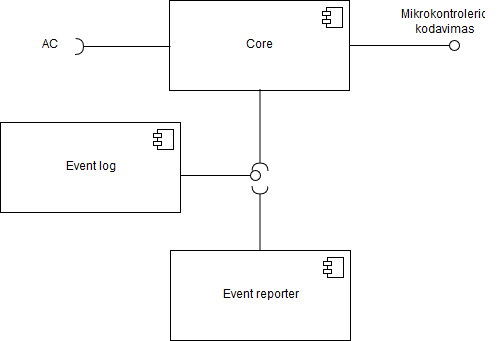
\includegraphics[width=10cm,height=10cm,keepaspectratio]{L2(mikrokontroleris).png}
	\caption{}
	\label{}
	\end{figure}

\item L2(Mikrokontroleris): Core(25 pav) įgyvendina Mikro kontrolerio kuriamą interfeisą, per kurį sistema ir turi galimybę koduoti patį mikro kontrolerį. Sistema gautus duomenis iš kontrolerio įrašo į Event log'ą.
\end{itemize}

\pagebreak

\subsection{Use case}
\begin{itemize}
\item Diagramoje (26 pav) pavaizduoti visi galimi veiksmai, kuriuos gali atlikti kiekvienas programos vartotojas.
		\begin{figure}[H]
		\centering	
	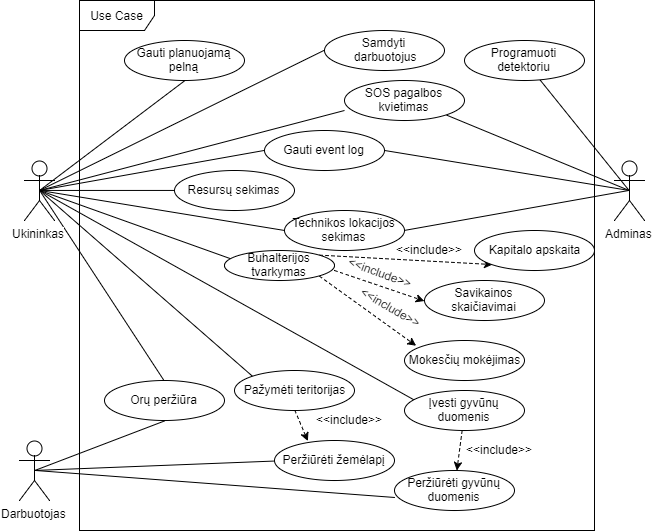
\includegraphics[width=15cm,height=17cm,keepaspectratio]{UseCaseFull.png}
	\caption{}
	\label{fig:UseCaseFull}
\end{figure}
\end{itemize}

\pagebreak

\subsection{Proceso pjūvis}
Šiame skyriuje pagrinde koncentruojamasi į programos elgseną jos vykdymo metu.
\subsubsection{Sekų diagramos}
\begin{itemize}
\item Diagramoje (27 pav)  pavaizduota seka, kurią programa atlieka Ukininkui norint gauti planuojamą jo pasirinkto laikotarpio pelną.
		\begin{figure}[H]
		\centering	
	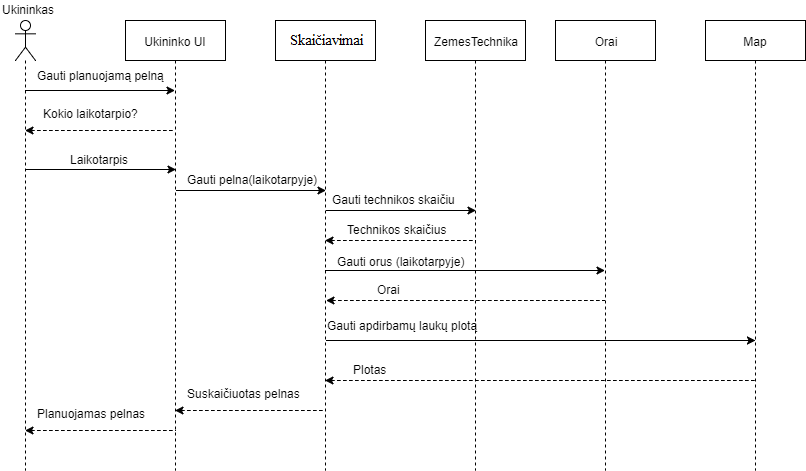
\includegraphics[width=17cm,height=20cm,keepaspectratio]{PelnoSkaičiavimas.png}
	\caption{}
	\label{fig:PelnoSkaičiavimas}
\end{figure}
Šioje diagramoje(27 pav) matome, kad ūkininkui pateikus užklausą planuojamui pelnui gauti, Ūkininkas UI kreipiasi į Calculations klasę su prašymu jį apskaičiuoti. Ši savo ruožtu norėdama gauti reikiamus duomenis kreipiasi į klases UkioTechnika, Map ir Orai.

\pagebreak

\item Teritorijos žimėjimo seka(28pav):
	\begin{figure}[H]
		\centering	
	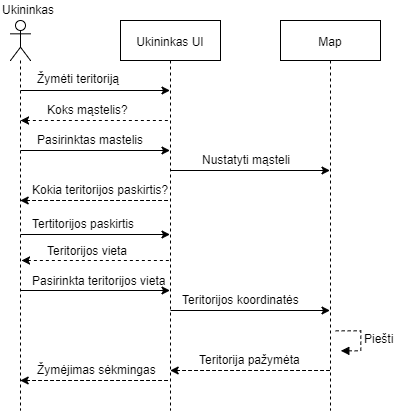
\includegraphics[width=10cm,height=10cm,keepaspectratio]{ŽymėtiTeritorijas.png}
	\caption{}
	\label{fig:ŽymėtiTeritorijas}
\end{figure}

\end{itemize}
\subsubsection{Būsenų diagramos}
\begin{itemize}
\item Detektoriaus būsenų diagrama(29 pav):

		\begin{figure}[H]
		\centering	
	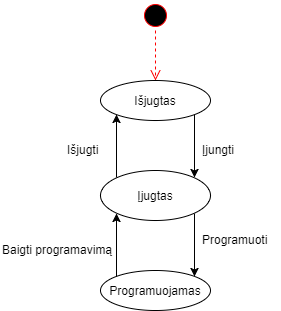
\includegraphics[width=7cm,height=7cm,keepaspectratio]{BusenuDetektorius.png}
	\caption{}
	\label{fig:BusenuDetektorius}
\end{figure}

\end{itemize}
Iš šios(29 pav) diagramos  matome, kad detektorius negali būt išjungtas programavimo metu, kad nekiltų klaidos vėlesnių paleidimų metu.
\subsubsection{Veiklos diagramos}
\begin{itemize}
\item Orų sekimo veiklos diagrama(30 pav):
	\begin{figure}[H]
	\centering	
	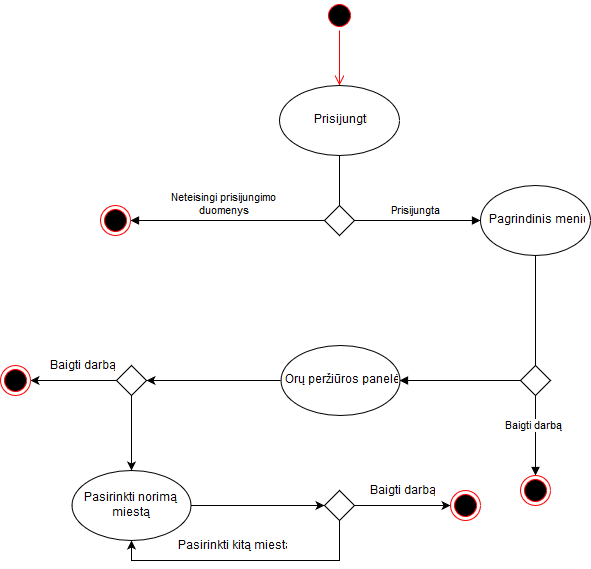
\includegraphics[width=10cm,height=10cm,keepaspectratio]{veiklos_diagrama_orai.png}
	\caption{}
	\label{}
	\end{figure}
\item Ūkio technikos sekimo veiklos diagrama(31 pav):
	\begin{figure}[H]
	\centering	
	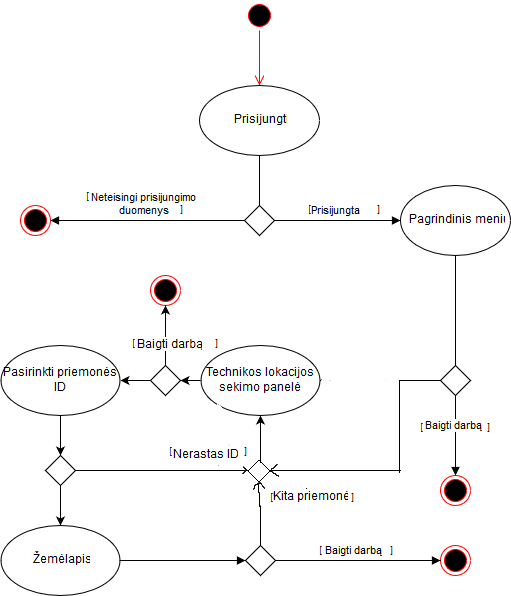
\includegraphics[width=10cm,height=10cm,keepaspectratio]{veiklos_diagrama_technikos_sekimas.png}
	\caption{}
	\label{}
	\end{figure}
\item Teritorijos žymėjimo veiklos diagrama(32 pav):
	\begin{figure}[H]
	\centering	
	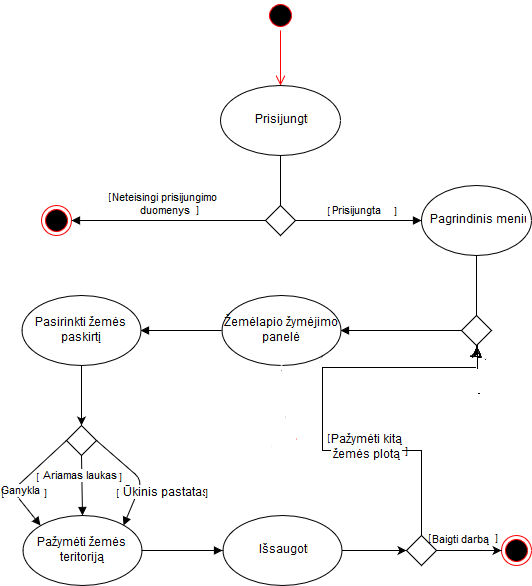
\includegraphics[width=10cm,height=10cm,keepaspectratio]{veiklos_diagrama_zymeti_teritorijas.png}
	\caption{}
	\label{}
	\end{figure}
\item Gyvūnų suvedimo veiklos diagrama(33 pav):
	\begin{figure}[H]
	\centering	
	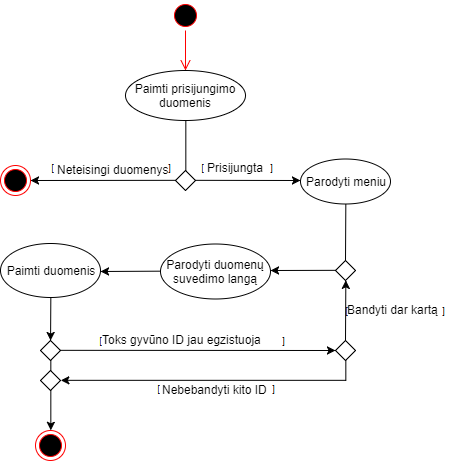
\includegraphics[width=10cm,height=10cm,keepaspectratio]{VeiklosGyvunuSuvedimas.png}
	\caption{}
	\label{}
	\end{figure}
\item Šiose diagramose matoma, kaip įgyvendinamas atitinkamas scenarijus programos vykdymo metu.
\end{itemize}
\subsection{Fizinis pjūvis}
	Šiame skyriuje parodoma programos naudojama aparatinė įranga, komunikacija tarp tinklo mazgų bei programos komponentų išdėstymas juose.
	\newline
	\vskip 0.5cm
	\begin{figure}[H]
	\centering	
	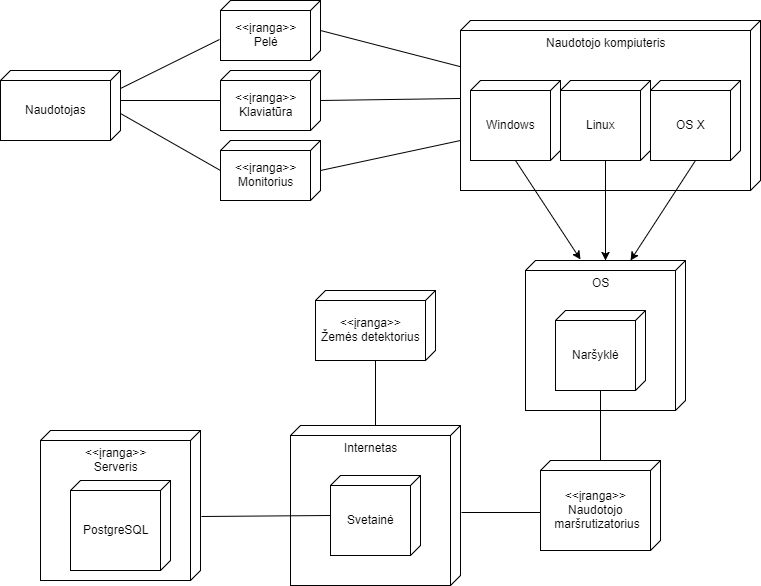
\includegraphics[width=15cm,height=15cm,keepaspectratio]{2D0.png}
	\caption{}
	\label{fig:Deployment}
\end{figure}
	\begin{itemize}
		\item D0: \hyperref[fig:Deployment]{\textit{Šioje diagramoje (34 pav.)}} parodyta, kaip išsaugomi programos duomenys. 
		Pirmoje projekto versijoje visi duomenys buvo saugomi kompiuteryje, vienintelis ryšys su internetu buvo per gismeteo.lt svetainę. Dabartinėje versijoje implementuotas duomenų saugojimas PostgreSQL duombazėje. Šioje diagramoje vaizduojamas kelias nuo naudotojo iki pasirinktos duombazės, naudojami techniniai įrenginiai ir jų sąryšiai su programinė įranga. Taip pat pridėtas žemės detektorius, kuris siunčia programai pasirinkto žemės ploto parametrų duomenis. Informacija, gauta iš žemės detektoriaus, taip pat talpinama PostgreSQL duombazėje.
	\end{itemize}

\pagebreak
\subsection{Antros dalies išvada}
Sistema suprojektuota tokiais principais, kad ją būtų lengva papildyti. Klasių dizainas atitinka Top->Bottom principą, kuris leidžia nesunkiai pridėti naujo funkcionalumo visai sistemai. Šis principas persikelia ir į kūrimo pjūvį. Sistemos įgyvendinami ir kuriami interfeisai yra labai moduliarūs ir nesunku pridėti ar išimti interfeisus iš sistemos. Vidinė programos struktūra sekų diagramoje aiškiai apibrėžia vartotojų sąveiką su sistema. Sekos išskirstytos diskrečiais ir aiškiais veiksmais, kas sumažina klaidų skaičių rašant kodą ir padeda suprasti, kaip viskas veikia. Iš fizinės pusės sistema yra serveryje ir dėl pasirinktos JAVA programavimo kalbos sistemą galimą pasileisti iš visų operacinių sistemų. Visa sistema yra serveryje. Duomenims saugoti psirinkome PostgreSQL, nes tai populiariausia nemokama duomenų bazių valdymo sistema. Sistemai yra vietos tobulėti. Ateityje egzistuoja galimybė ją pritaikyti išmaniesiams telefonams bei kitiems nešiojamiems įrenginiams.



\sectionnonum{Rezultatai ir išvados}
Projektuodami tą pačią sistemą du kartus skirtingais būdais pamatėme aiškius stilių skirumus. Kuriant sistemą nesilaikant jokių aiškių principų, kodas ir pati sistemos struktūra tampa neaiški, po kiek laiko prisimeni apie neįgyvendintus funkcionalumus arba idėjas, kurias įdėti į sistemą būtų labai sunku. Projektuojant sistemą antrą kartą buvo prisilaikyta Top->Bottom ir OOP principų, kurie leido lengviau struktūrizuoti visą darbą. Klasių ir komponentų diagramos pasidarė aiškiai suprantamos ir nauji funkcionalumai būtų nesunkiai įgyvendinami ateityje. Buvo aiškiau apibrėžtas fizinis sistemos principas, leidžiantis lanksciau naudotis sistema. Deja, ne viską pavyko pridėti. Norėtųsi įdėti išmaniojo telefono palaikymą mūsų sistemoje, bet dėl laiko stokos to nebepadarėme. Tačiau tikime, kad dėl struktūros pranašumų tai padaryti nebūtų sunku. Išmokome fundamentalius PSI aspektus, UML diagramų braižymą, išmokome naudotis keletu UML braižymo programų ir .pdf failų kurimo programa Latex, kuri palengvino darbą komandoje. Dėl gero darbų pasidalijimo projekto kūrimas vyko sklandžiai. 




\end{document}
